\documentclass[conference]{IEEEtran}
\usepackage[utf8]{inputenc}
\usepackage[T1]{fontenc}
\usepackage[brazil]{babel}
\usepackage{amsmath}
\usepackage{graphicx}
\usepackage{booktabs}
\usepackage{url}
\usepackage{listings}
\usepackage{xcolor}

\lstset{basicstyle=\ttfamily\footnotesize, breaklines=true, frame=single, columns=fullflexible,
  commentstyle=\color{gray}, morecomment=[l]{//},
  literate={á}{{\'a}}1 {à}{{\`a}}1 {ã}{{\~a}}1 {â}{{\^a}}1 {é}{{\'e}}1 {ê}{{\^e}}1 {í}{{\'i}}1 {ó}{{\'o}}1
           {õ}{{\~o}}1 {ô}{{\^o}}1 {ú}{{\'u}}1 {ç}{{\c{c}}}1 {Á}{{\'A}}1 {É}{{\'E}}1 {Ç}{{\c{C}}}1
           {→}{{$\rightarrow$}}1 {←}{{$\leftarrow$}}1 {×}{{$\times$}}1 {·}{{$\cdot$}}1 {θ}{{$\theta$}}1}

\begin{document}
\title{Desenvolvimento de uma Engine Gráfica 2D com Editor Visual \\ para Renderização e Iluminação de Sprites com OpenGL}
\author{\IEEEauthorblockN{Pedro Paulo Santos de Jesus Junior -- Luiz Filipe Chiarinotti}
\IEEEauthorblockA{\textit{Engenharia de Computação} \\ \textit{FHO -- Fundação Hermínio Ometto}\\ Araras, Brasil \\ RA 113538 -- RA 113079}}
\maketitle
\begin{abstract}
This paper presents a 2D graphics engine for sprite rendering written in Python with OpenGL 3.3, together with a visual editor inspired by Unity. The engine organizes the scene as game objects with components and supports PNG textures with alpha blending, homogeneous transformations, a hierarchy of transforms, draw order by sorting layers, instanced batch rendering, 2D lighting with stencil shadow volumes, physics with gravity and a tile map editor. Following the research axis of real-time visualization of large models, view frustum culling was adapted from 3D CAD/BIM scenes to 2D. Experiments show that batching sprites by texture reduces the frame time about five times, that culling discards up to 98\% of the sprites in large worlds, and that each light costs about 0.1 ms per frame. Six game projects were built with the engine.
\end{abstract}
\begin{IEEEkeywords}
Computação Gráfica, Engine 2D, OpenGL, Sprites, Iluminação 2D, Sombras, Frustum Culling, Editor de Cenas
\end{IEEEkeywords}
\section*{Resumo}
Este trabalho apresenta uma engine gráfica 2D para renderização de sprites, escrita em Python com OpenGL 3.3, acompanhada de um editor visual inspirado na Unity. A engine organiza a cena em objetos com componentes e oferece texturas PNG com transparência, transformações em coordenadas homogêneas, hierarquia de objetos, ordem de desenho por camadas, desenho em lote com \textit{instancing}, iluminação 2D com sombras por \textit{stencil}, física com gravidade e um editor de mapas por blocos. Seguindo o eixo de visualização em tempo real de modelos grandes, o \textit{view frustum culling} de cenas CAD/BIM foi adaptado para 2D. Os testes mostraram que agrupar sprites por textura reduz o tempo de cada quadro em cerca de cinco vezes, que o \textit{culling} descarta até 98\% dos sprites em mundos grandes e que cada luz custa cerca de 0,1 ms por quadro.

\section{Introdução}
Motores gráficos organizam as operações necessárias para gerar imagens em tempo real: carregar texturas, representar os objetos, aplicar transformações, decidir a ordem de desenho e calcular a iluminação. Ferramentas como a Unity escondem essas etapas atrás de um editor visual. Construir uma engine própria permite estudar o que existe por trás dessas abstrações.
Este trabalho apresenta uma engine exclusivamente 2D, escrita em Python com OpenGL 3.3. A unidade básica de desenho é o \textit{sprite}: uma imagem aplicada como textura sobre um quadrilátero, com posição, rotação, escala e uma ordem de desenho. A engine é organizada como a Unity: a cena é formada por objetos com um \textit{Transform} e uma lista de componentes, e um editor visual permite montar as cenas com o mouse. Além do desenho de sprites, foram implementados iluminação 2D com sombras, física com gravidade e um editor de mapas por blocos.
O trabalho se insere no \textbf{Eixo 2 (Engenharia Civil e Modelação CAD)}: a técnica de descarte de objetos fora do campo de visão, estudada para visualizar modelos BIM em tempo real, foi adaptada para uma engine 2D de jogos com milhares de sprites. O objetivo geral é desenvolver uma engine capaz de instanciar, transformar, organizar, iluminar e renderizar sprites em tempo real; os objetivos específicos são implementar as texturas, as transformações e a ordem de desenho, o pipeline com desenho em lote, o \textit{frustum culling} 2D, a iluminação com sombras e o editor, e medir o desempenho.

\section{Trabalhos Relacionados}
O OpenGL fornece acesso ao pipeline gráfico: os vértices são processados por um \textit{vertex shader}, rasterizados e coloridos por um \textit{fragment shader} \cite{segal2010,akenine2018}. Em 2D, os sprites são quadriláteros texturizados que reutilizam a mesma geometria. Engines de jogos organizam a cena com objetos e componentes de transformação, renderização e lógica \cite{gregory2018}.
Johansson, Roupé e Bosch-Sijtsema \cite{johansson2015} mostram que modelos BIM com milhares de objetos só são visualizados em tempo real com técnicas que evitam enviar à GPU o que não está visível, como o \textit{frustum culling} e a redução de chamadas de desenho. Assarsson e Möller \cite{assarsson2000} descrevem testes rápidos do volume envolvente contra a pirâmide de visão, e a ideia de organizar a cena para descartar regiões vem de Clark \cite{clark1976}.
Para as sombras, Crow \cite{crow1977} propôs os volumes de sombra, e Heidmann \cite{heidmann1991} mostrou como calculá-los em tempo real com o \textit{stencil buffer}. Neste trabalho a mesma ideia é aplicada em 2D. Na física, a grade espacial \cite{teschner2003,ericson2005} reduz os pares de objetos testados.

\section{Metodologia e Modelagem Computacional}

\subsection{Arquitetura Geral}
A engine usa Pygame para a janela e a entrada, PyOpenGL para o OpenGL 3.3 e NumPy para cálculos vetorizados. Os módulos principais são o motor (loop), a cena, os objetos e componentes, as texturas, o renderizador, a física, a interface e o editor. A cada quadro o motor processa os eventos, atualiza os componentes, executa a física, copia as poses dos objetos para os sprites, monta o mapa de luz, ordena e descarta os sprites invisíveis, desenha e apresenta a imagem.

\subsection{Sprites e Transformações}
Cada sprite é representado por
\begin{equation}
S = \{T_x, T_y, \theta, S_x, S_y, L, I\}
\end{equation}
onde Tx e Ty são a posição, $\theta$ a rotação, Sx e Sy a escala, L a ordem de desenho e I a textura. A geometria é um quadrilátero de dois triângulos, guardado uma única vez num \textit{vertex buffer} e compartilhado por todos os sprites. Imagens PNG são carregadas com o canal alfa e combinadas por \textit{alpha blending}. A matriz de modelo, em coordenadas homogêneas, é calculada na forma fechada:
\begin{equation}
M = T \cdot R \cdot S =
\begin{bmatrix}
S_x\cos\theta & -S_y\sin\theta & T_x\\
S_x\sin\theta & S_y\cos\theta & T_y\\
0 & 0 & 1
\end{bmatrix}
\end{equation}
Objetos podem ser filhos de outros; a pose no mundo é a composição com a do pai, M\_mundo = M\_pai $\cdot$ M\_local. Assim, o farol de uma nave ou o céu filho da câmera acompanham o pai.

\subsection{Ordem de Desenho}
Como os sprites têm transparência, não é usado \textit{z-buffer}: a ordem vem de uma lista ordenada pela chave (camada de desenho, ordem na camada, posição na hierarquia). As camadas de desenho são uma lista definida no projeto (por exemplo, Fundo, Cenário, Padrão e Frente); havendo empate, o objeto que vem depois na hierarquia é desenhado por cima. A ordenação é estável e só é refeita quando algum sprite entra, sai ou muda de camada.

\subsection{Pipeline de Renderização e Desenho em Lote}
No modo \textit{individual}, cada sprite gera uma chamada de desenho com sua matriz enviada ao \textit{vertex shader}. Como cada chamada do Python ao OpenGL é cara, foram implementados também: \textbf{lote}, em que sprites vizinhos com a mesma textura viram uma chamada instanciada (\texttt{glDrawArraysInstanced}), com as matrizes de todos calculadas de uma vez no NumPy e enviadas num buffer de instâncias; \textbf{lote agrupado}, que ordena por textura dentro da mesma camada; e \textbf{atlas}, que reúne as imagens numa textura e desenha a cena inteira numa chamada. Os lotes também são separados pelo modo de mistura (normal ou aditivo).
\begin{figure}[htbp]
\centerline{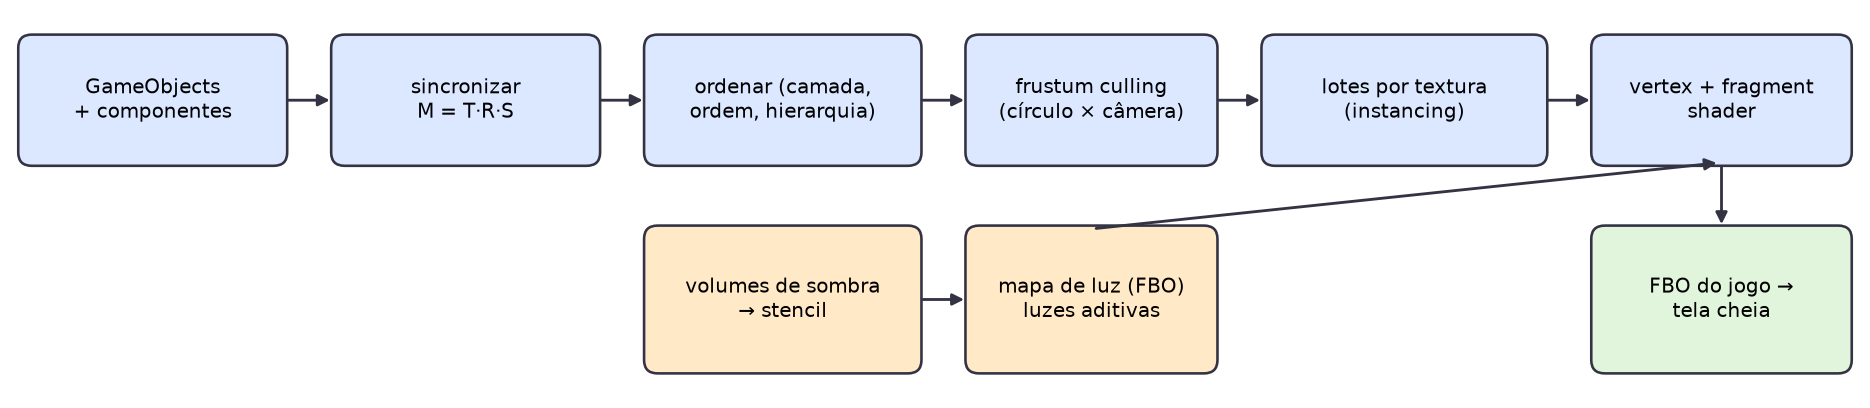
\includegraphics[width=\columnwidth]{figuras/pipeline.png}}
\caption{Pipeline da engine: preparação dos sprites (azul), iluminação (laranja) e tela cheia (verde).}
\label{fig:pipeline}
\end{figure}

\subsection{Adaptação do Frustum Culling para 2D}
Em 3D, o \textit{frustum} é a pirâmide de visão da câmera \cite{assarsson2000}. Em 2D ele se reduz ao retângulo visível, de centro (cx, cy) e meias dimensões
\begin{equation}
h_w = \frac{W}{2z}, \qquad h_h = \frac{H}{2z}
\end{equation}
onde W $\times$ H é a área de desenho e z o zoom. Cada sprite é envolvido por um círculo de raio r = $\frac{1}{2}$$\cdot$$\sqrt{}$((w$\cdot$Sx)$^2$ + (h$\cdot$Sy)$^2$) e é descartado quando
\begin{equation}
|x - c_x| > h_w + r \quad \text{ou} \quad |y - c_y| > h_h + r .
\end{equation}
O teste é feito para todos os sprites de uma vez, de forma vetorizada, antes do desenho.

\subsection{Iluminação 2D com Sombras}
Os componentes \textit{Luz2D} (luz global, pontual ou em cone) e \textit{ProjetorSombra2D} (objeto que bloqueia a luz) definem a iluminação. A cada quadro, as luzes são desenhadas num \textbf{mapa de luz}: um \textit{framebuffer} do tamanho da tela, com textura em ponto flutuante (RGBA16F) e \textit{stencil}, limpo com a cor da luz global. Cada luz é um quadrilátero desenhado com mistura aditiva, cujo \textit{fragment shader} calcula a atenuação
\begin{equation}
a(d) = \left(1 - \mathrm{smoothstep}(d_0, 1, d)\right)^2
\end{equation}
onde d é a distância ao centro dividida pelo raio e d0 o raio interno; na luz em cone, a atenuação é multiplicada por uma transição suave do ângulo entre o pixel e a direção da luz.
As sombras usam volumes de sombra 2D \cite{crow1977,heidmann1991}. Para cada objeto próximo de uma luz, são geradas as retas tangentes que partem da luz e tocam o círculo do objeto (ou as arestas da caixa voltadas para longe da luz), estendidas para longe. Esses triângulos são desenhados apenas no \textit{stencil buffer}, e a luz é então desenhada somente onde o \textit{stencil} continuou zero. Por fim, o \textit{fragment shader} dos sprites lê o mapa de luz na posição do pixel (\texttt{gl\_FragCoord}) e multiplica a cor; sprites marcados como sem luz (tiros, estrelas) e sprites aditivos (fogo, explosões) mantêm o brilho próprio Fig.~\ref{fig:luz}.
\begin{figure}[htbp]
\centerline{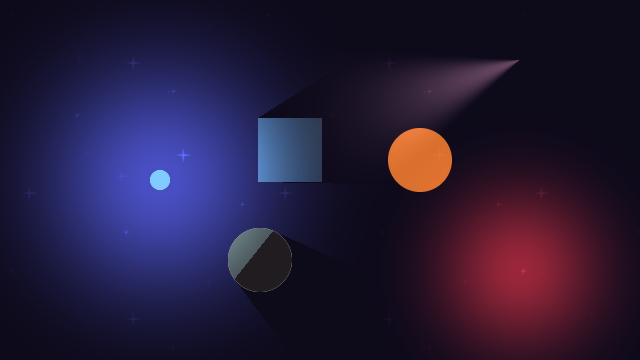
\includegraphics[width=\columnwidth]{figuras/luz.png}}
\caption{Teste da iluminação: luz azul com sombras de uma caixa e de um círculo, luz vermelha, luz em cone e sprites com brilho próprio.}
\label{fig:luz}
\end{figure}

\subsection{Framebuffers, Física e Recursos de Cena}
Para a tela cheia, o jogo é desenhado num \textit{framebuffer} na sua resolução, e esse quadro é ampliado para o monitor mantendo a proporção. A interface é desenhada numa superfície do Pygame e enviada como textura com \texttt{glTexSubImage2D}, sem cópia na CPU.
A física tem corpos dinâmicos (com gravidade), cinemáticos e estáticos, colisores em círculo ou caixa e plataformas atravessáveis por baixo. A fase ampla usa grade espacial; a fase estreita calcula o vetor mínimo de separação, que afasta os corpos e anula a velocidade contra a superfície. O passo é dividido em subpassos quando algo se move rápido, e há consultas por raio. A cena também oferece partículas, fundos com paralaxe e mapas de blocos, cujos blocos sólidos são unidos em poucos retângulos de colisão.

\subsection{Editor}
O editor Fig.~\ref{fig:editor} segue o layout da Unity: \textit{Hierarchy} (arrastar reordena ou cria filhos), \textit{Scene} com ferramentas de mover, girar e escalar e visualização das luzes, \textit{Inspector}, \textit{Project} e \textit{Console}. Scripts Python são criados e recarregados pelo editor, prefabs são criados arrastando objetos para o projeto, e mapas de blocos são pintados diretamente na cena com uma paleta. As cenas são salvas em JSON. Para os testes, um robô injeta eventos reais de mouse e teclado e usa o editor como uma pessoa; dois dos jogos foram montados dessa forma.
\begin{figure}[htbp]
\centerline{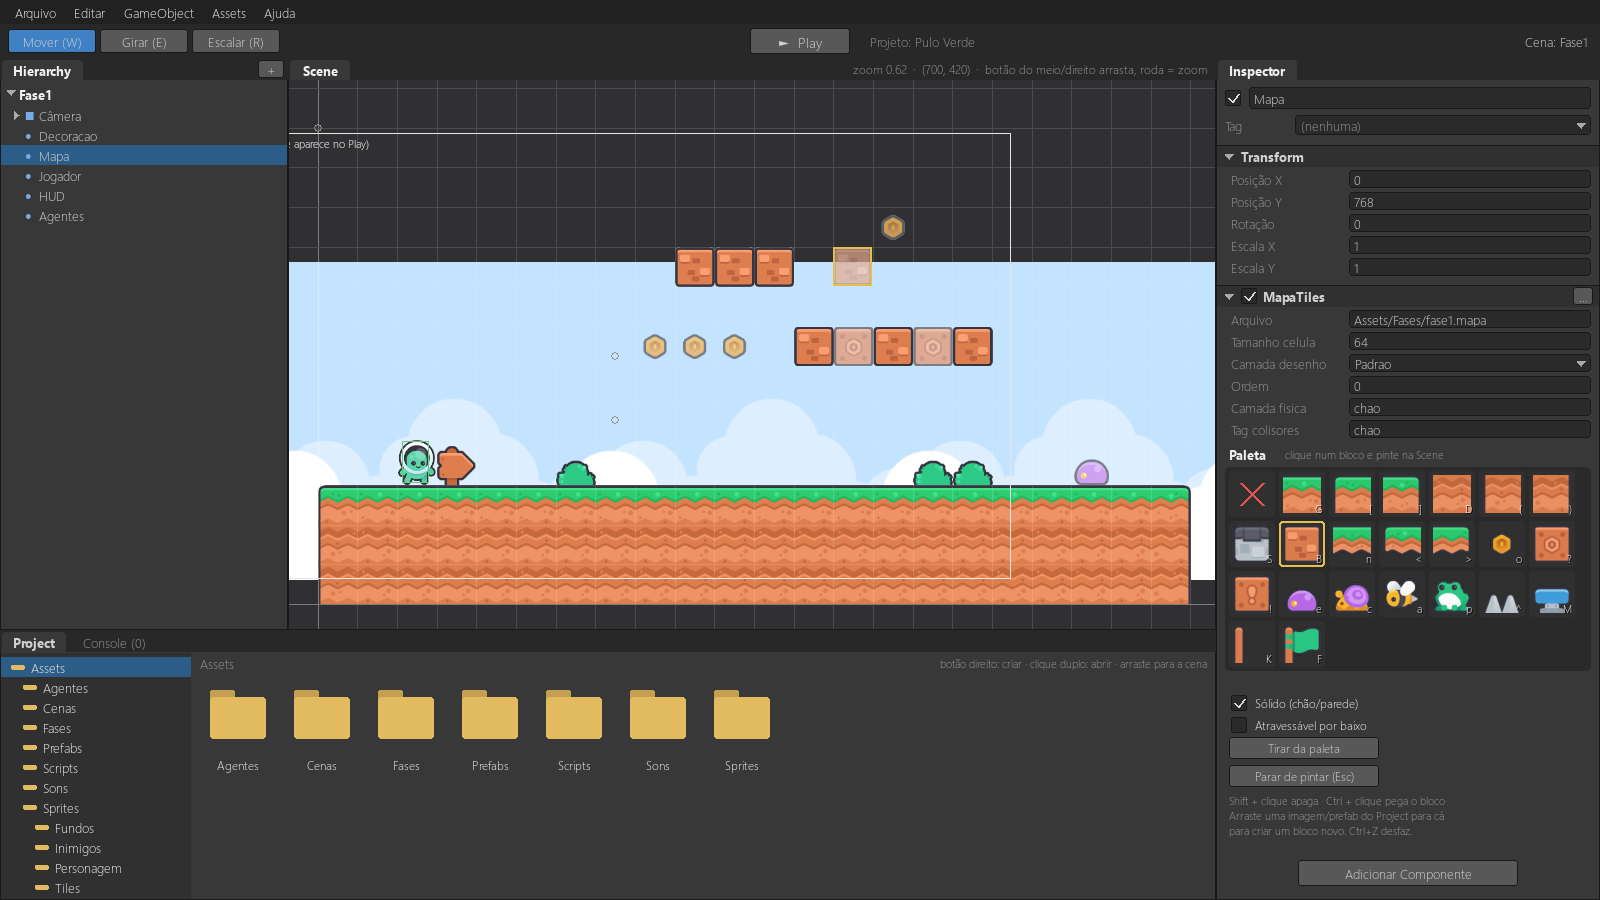
\includegraphics[width=\columnwidth]{figuras/paleta.png}}
\caption{Editor da engine: Hierarchy, Scene (pintando blocos da fase), Inspector com a paleta e Project.}
\label{fig:editor}
\end{figure}

\section{Resultados e Avaliação de Desempenho}
Os testes foram feitos num notebook com GPU integrada AMD Radeon Vega 8, Python 3.13 e janela de 1280 $\times$ 720, sem sincronização vertical. Cada caso mediu centenas de quadros, com \texttt{glFinish} para incluir o tempo da GPU.
A Tabela~\ref{tab:modos} mostra o tempo por quadro nos quatro modos. O custo é dominado pelas chamadas OpenGL feitas pelo Python: no lote com texturas misturadas quase não há agrupamento, e ele chega a ser mais lento que o individual. Agrupando por textura ou usando atlas, as chamadas caem para 20 ou 1 e o tempo cai cerca de cinco vezes. A resolução da janela quase não alterou o tempo, indicando que o gargalo é a CPU.
\begin{table}[htbp]
\caption{Tempo médio por quadro (ms) por modo de desenho}
\begin{center}
\begin{tabular}{rrrrr}
\toprule
Sprites & Individual & Lote & Agrupado & Atlas \\
\midrule
1 000 & 33,3 & 41,2 & 8,1 & 8,2 \\
5 000 & 153 & 187 & 27,8 & 25,3 \\
20 000 & 596 & 746 & 116 & 118 \\
\bottomrule
\end{tabular}
\label{tab:modos}
\end{center}
\end{table}
A Tabela~\ref{tab:culling} mostra o \textit{culling} com 20 000 sprites em mundos de tamanho crescente. Com tudo na tela, o teste só acrescenta custo; a partir de um mundo de 2 $\times$ 2 telas ele compensa, chegando a descartar 98\% dos sprites.
\begin{table}[htbp]
\caption{Frustum culling com 20 000 sprites}
\begin{center}
\begin{tabular}{lrrr}
\toprule
Mundo & Sem culling & Com culling & Descartados \\
\midrule
1 $\times$ 1 & 108,8 ms & 142,2 ms & 0\% \\
2 $\times$ 2 & 98,7 ms & 81,4 ms & 73\% \\
4 $\times$ 4 & 101,0 ms & 69,1 ms & 93\% \\
8 $\times$ 8 & 100,6 ms & 66,8 ms & 98\% \\
\bottomrule
\end{tabular}
\label{tab:culling}
\end{center}
\end{table}
A Tabela~\ref{tab:luzes} mostra o custo da iluminação com 2 000 sprites. Cada luz sem sombra acrescenta cerca de 0,1 ms por quadro, pois é um único quadrilátero desenhado pela GPU; com sombras de 40 objetos, cada luz custa cerca de 0,3 ms, por causa do cálculo dos volumes na CPU e das passagens pelo \textit{stencil}.
\begin{table}[htbp]
\caption{Custo da iluminação 2D (2 000 sprites)}
\begin{center}
\begin{tabular}{rrrr}
\toprule
Luzes & Sem sombra & Com sombra & Triângulos \\
\midrule
0 & 34,0 ms & --- & 0 \\
10 & 34,4 ms & 38,2 ms & 160 \\
50 & 38,5 ms & 51,0 ms & 890 \\
100 & 43,0 ms & 62,5 ms & 1 646 \\
200 & 53,1 ms & 98,8 ms & 3 720 \\
\bottomrule
\end{tabular}
\label{tab:luzes}
\end{center}
\end{table}
Na física, a grade espacial testou 1 976 pares com 2 000 objetos, contra 1 999 000 numa comparação de todos contra todos. A engine tem 110 testes automáticos, que verificam as transformações, a ordem de desenho, a física, a iluminação (medindo pixels da imagem) e o editor. Com ela foram feitos seis projetos de jogo, entre eles um \textit{shoot 'em up} com iluminação e sombras Fig.~\ref{fig:navinha} e um jogo de plataforma.
\begin{figure}[htbp]
\centerline{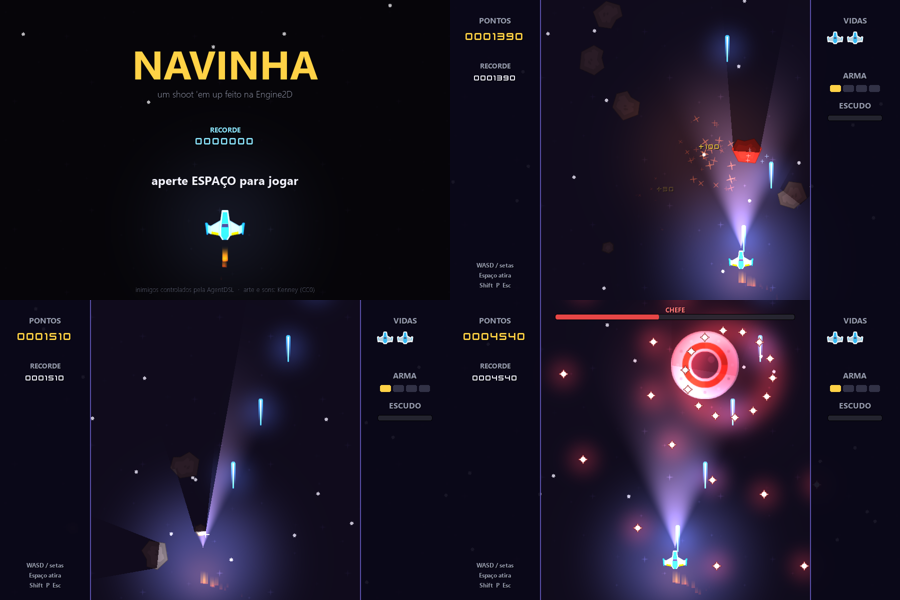
\includegraphics[width=\columnwidth]{figuras/navinha_iluminacao.png}}
\caption{Jogo feito com a engine: farol da nave com sombras dos meteoros, clarões das explosões e a luz do chefe.}
\label{fig:navinha}
\end{figure}

\section{Conclusão e Trabalhos Futuros}
Foi desenvolvida uma engine 2D com os componentes fundamentais de um motor gráfico --- texturas, sprites, transformações, ordem de desenho e pipeline de renderização ---, acrescida de iluminação com sombras por \textit{stencil}, física e um editor visual. A adaptação do \textit{frustum culling} de cenas BIM para 2D mostrou ganho quando a maior parte da cena está fora da tela, e o desenho em lote foi a otimização de maior impacto.
A principal limitação é o Python, que torna caras a atualização de muitos objetos e as chamadas gráficas. Como trabalhos futuros, propõem-se mover a atualização dos sprites e o cálculo das sombras para a GPU, uma estrutura espacial hierárquica para o \textit{culling}, mapas normais para a iluminação e a exportação de jogos executáveis.

\begin{thebibliography}{00}
\bibitem{segal2010} M. Segal and K. Akeley, ``The OpenGL Graphics System: A Specification (Version 3.3 Core Profile),'' Khronos Group, 2010.
\bibitem{akenine2018} T. Akenine-Möller, E. Haines and N. Hoffman, \textit{Real-Time Rendering}, 4th ed. Boca Raton: CRC Press, 2018.
\bibitem{gregory2018} J. Gregory, \textit{Game Engine Architecture}, 3rd ed. Boca Raton: CRC Press, 2018.
\bibitem{johansson2015} M. Johansson, M. Roupé and P. Bosch-Sijtsema, ``Real-time visualization of building information models (BIM),'' \textit{Automation in Construction}, vol. 54, pp. 69--82, 2015.
\bibitem{assarsson2000} U. Assarsson and T. Möller, ``Optimized view frustum culling algorithms for bounding boxes,'' \textit{Journal of Graphics Tools}, vol. 5, no. 1, pp. 9--22, 2000.
\bibitem{clark1976} J. H. Clark, ``Hierarchical geometric models for visible surface algorithms,'' \textit{Communications of the ACM}, vol. 19, no. 10, pp. 547--554, 1976.
\bibitem{crow1977} F. C. Crow, ``Shadow algorithms for computer graphics,'' \textit{ACM SIGGRAPH Computer Graphics}, vol. 11, no. 2, pp. 242--248, 1977.
\bibitem{heidmann1991} T. Heidmann, ``Real shadows, real time,'' \textit{IRIS Universe}, no. 18, pp. 28--31, 1991.
\bibitem{teschner2003} M. Teschner, B. Heidelberger, M. Müller, D. Pomeranets and M. Gross, ``Optimized spatial hashing for collision detection of deformable objects,'' in \textit{Proc. Vision, Modeling, and Visualization (VMV)}, 2003, pp. 47--54.
\bibitem{ericson2005} C. Ericson, \textit{Real-Time Collision Detection}. San Francisco: Morgan Kaufmann, 2005.
\end{thebibliography}

\end{document}
